\documentclass[11pt, a4paper]{article}
\usepackage{graphicx}
\usepackage{amsmath}
\usepackage{listings}
\usepackage{minted}
\usepackage{physics}

\title{EE2703 Applied Programming Lab - Assignment No 7}
\author{
  \textbf{Name}: Atishay Ganesh\\
  \textbf{Roll Number}: EE17B155
}\date{\today}
\begin{document}
		
\maketitle 
\section{Abstract}
The goal of this assignment is the following.
\begin{itemize}
\item To analyze Filters using Laplace Transform.
\item To see how python can be used for symbolic Algebra.
\item To plot graphs to understand high pass and low pass analog filters.
\end{itemize}
\usemintedstyle{manni}

\section{Assignment}
\subsection{Setting up the variables}
Importing the standard libraries
\begin{minted}[mathescape,escapeinside = ||]{python3}
import numpy as np
import matplotlib.pyplot as plt
import matplotlib
import scipy.signal as sp
from sympy import *
\end{minted}
We initialize sympy and define a plotting function to help simplify the code.
\begin{minted}{python3}
init_printing()
s = symbols('s')
plt.rcParams.update({'mathtext.default':  'regular' })

def plotter(fig_no,arg1,arg2,label_x,label_y,type=plt.plot,arg3='b-',title="",cmap = matplotlib.cm.jet):
    plt.figure(fig_no)
    plt.grid(True)
    if type==plt.contourf:
        type(arg1,arg2,arg3,cmap=cmap)
        plt.colorbar()
    else:
        type(arg1,arg2,arg3)
    plt.xlabel(label_x,size =19)
    plt.ylabel(label_y,size =19)
    plt.title(title)

\end{minted}

We also define a function to make bode plots.
\begin{minted}{python3}
def bodeplot(figure,H):
    plt.figure(figure)
    w,s,phi = H.bode()
    plt.subplot(2,1,1)
    plt.semilogx(w,s)
    plt.grid(True)
    plt.ylabel(r'$|H(j\omega)|$',size =17)
    plt.subplot(2,1,2)
    plt.semilogx(w,phi)
    plt.grid(True)
    plt.xlabel(r'$\omega$',size=17)
    plt.ylabel(r'$\angle(H(j\omega))$',size =17)

\end{minted}

\subsection{Defining the filters}
{
We write the matrix equation of the given two systems and use sympy to symbolically solve for the transfer functions.
}
\begin{minted}{python3}
def lowpass(R1,R2,C1,C2,G,Vi=1):
    '''Active 2nd order low pass butterworth filter using opamp''' 
    A = Matrix([[0,0,1,-1/G],[-1/(1+s*R2*C2),1,0,0],
                   [0,-G,G,1],[-1/R1-1/R2-s*C1,1/R2,0,s*C1]])
    b = Matrix([0,0,0,Vi/R1])
    V = A.inv()*b
    return(A,b,V)


def highpass(R1,R2,C1,C2,G,Vi = 1):
    '''Active 2nd order high pass filter using opamp'''
    A = Matrix([[0,0,1,-1/G],[-1/(1+1/(s*R2*C2)),1,0,0],
                [0,-G,G,1],[-s*C1-s*C2-1/R1,s*C2,0,1/R1]])
    b = Matrix([0,0,0,Vi*s*C1])
    V = A.inv()*b
    return(A,b,V)
\end{minted}

\subsection{Converting to scipy signals form}
{
We convert the transfer functions thus got to scipy signals form, which will help us in further calculations.
}
\begin{minted}{python3}
def simplifytoH(V):
    '''extracts H from the result of the matrix inversion'''
    Vo = V[3]
    #since the third element in the V column is actually the output voltage
    Vo = expand(simplify(Vo))#converting the simple rational form
    H = sympytoscipytf(Vo)
    return H

def sympytoscipytf(Vo):
    '''converts sympy tf to scipy tf'''
    v1 = fraction(Vo)#converting to numerator and denominator
    n,d = Poly(v1[0],s),poly(v1[1],s)
    numer,denom = n.all_coeffs(), d.all_coeffs()#extracting coeffs
    numer,denom = [float(f) for f in numer], [float(f) for f in denom]
    H = sp.lti(numer,denom)#converting to scipy lti form
    return H

A,b,V = lowpass(10000,10000,1e-8,1e-8,1.586,1)
'''We use 10 nF as it gives us nice figures'''
Hl = simplifytoH(V)
t = np.arange(0,1e-2,1e-7)
A,b,V = highpass(1e4,1e4,1e-9,1e-9,1.586)
'''We use 1 nF as it gives us nice values'''
Hh = simplifytoH(V)

\end{minted}

\subsection{Bode plots}
{
We draw bode plots of the filters, to verify indeed that they are low and high pass filters respectively.
}
\begin{minted}{python3}
#Drawing Bode Plots of the filters
bodeplot(0,Hl)
plt.title("Bode plot of lpf")
bodeplot(1,Hh)
plt.title("Bode plot of hpf")
plt.show()

\end{minted}
\begin{figure}[!tbh]
   	\centering
   	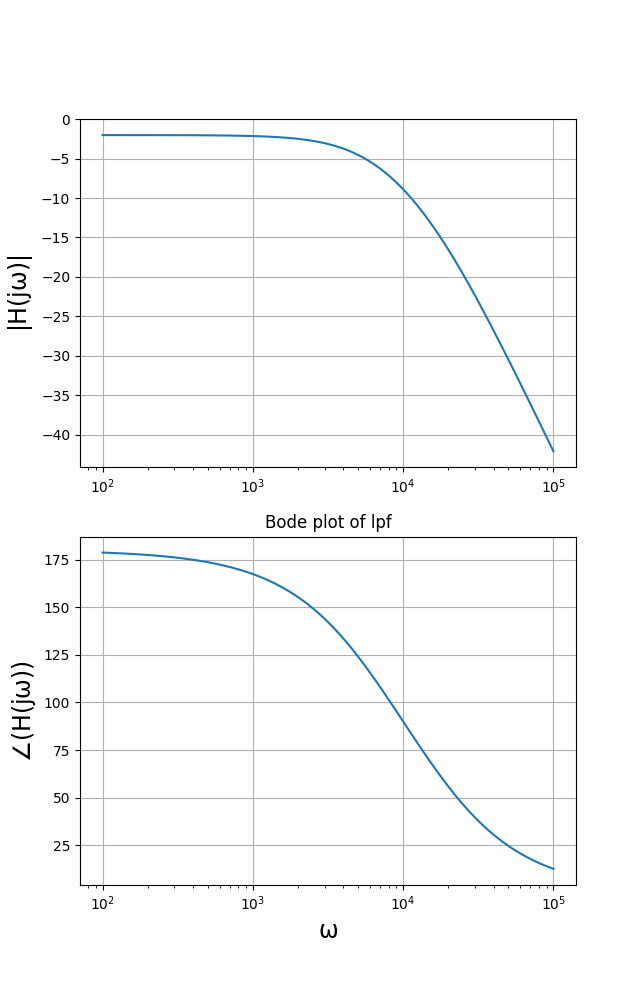
\includegraphics[scale=0.5]{img1.png}
   	\label{fig:32}
   \end{figure}
\begin{figure}[!tbh]
   	\centering
   	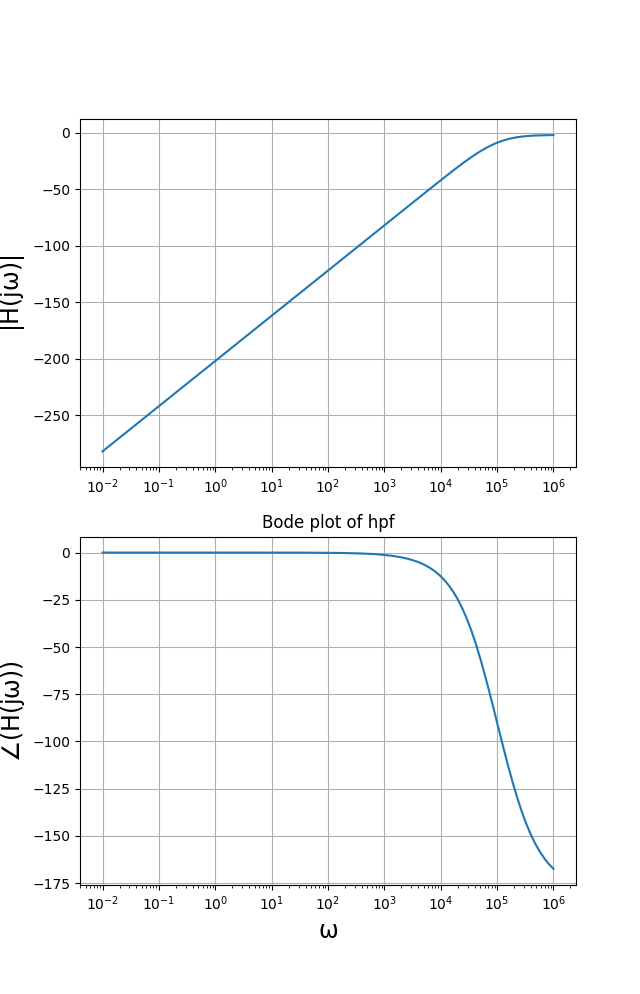
\includegraphics[scale=0.5]{img2.png}
   	\label{fig:32}
   \end{figure}

{ 
We observe that the impulse response of the first filter drops offs towards higher frequencies and that of the second filter increases towards higher frequencies, hence they are low and high pass filters respectively.
}
\subsection{Step Response}
{
We plot the step response of both the filters to see what it shows.
}
\begin{minted}{python3}
#Plotting step response of Analog filters
t,vtd,svec = sp.lsim(Hl,np.ones_like(t),t)
plotter(0,t,abs(vtd),r"t",r'Vo(t)',
       plt.loglog,title ='Response of lpf to unit step')

t,vtd,svec = sp.lsim(Hh,np.ones_like(t),t)
plotter(1,t,(vtd),r"t",r'Vo(t)',
       plt.semilogx,title ='Response of hpf to unit step')
plt.show()

\end{minted}
\begin{figure}[!tbh]
   	\centering
   	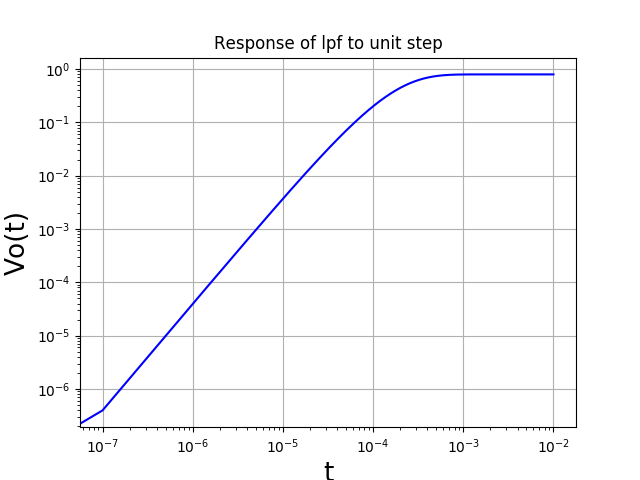
\includegraphics[scale=0.5]{img3.png}
   	\label{fig:32}
   \end{figure}
\begin{figure}[!tbh]
   	\centering
   	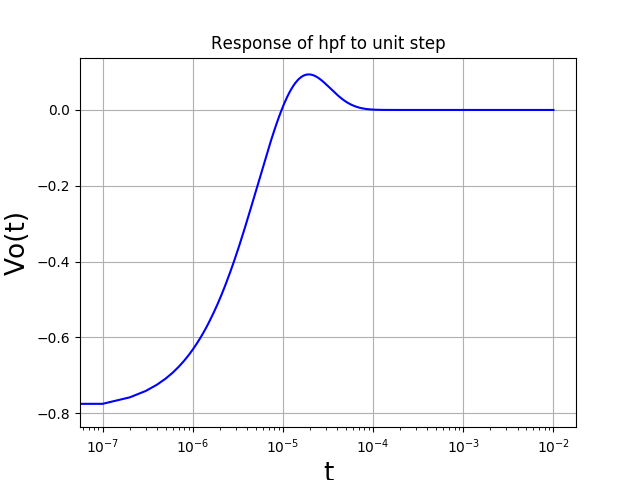
\includegraphics[scale=0.5]{img4.png}
   	\label{fig:32}
   \end{figure}
{

Using the initial and final value theorem, we understand the following.
\begin{itemize}
    \item The low pass filter's step response has a final value of about 0.79, indicating, it allows DC almost intact.
    \item The high pass filter's step response has a final value of 0, which shows it does not allow DC to pass through
    \item The low pass filter's step response has a initial value of 0, indicating, it does not allow high frequency AC to pass.
    \item The high pass filter's step response has a initial value of magnitude 0.79, which shows it does  allow high frequency AC to pass. 

    \item No overshoot in lpf case as it is a butterworth filter
    \item Overshoot is observed in hpf case.
\end{itemize}
}


\subsection{Response to sum of two sinusoids}
{
We plot the response of the filters to a sum of two input sinusoids.
}
\begin{minted}{python3}
#Response of high and low pass filter to sum of sinusoids.
#Frequency of one is in the pass band of lpf and stop band of hpf.
#Frequency of other is in the pass band of hpf and stop band of hpf.
t,vtd,svec = sp.lsim(Hl,(np.sin(2000*np.pi*t)+np.cos(2*10**6*np.pi*t)),t)
plotter(0,t,vtd,r"t",r'Vo(t)',
       plt.plot,title ='Response of lpf to sum of 2 sinusoids')
t,vtd,svec = sp.lsim(Hh,(np.sin(2000*np.pi*t)+np.cos(2*10**6*np.pi*t)),t)
plotter(1,t[0:500],vtd[0:500],r"t",r'Vo(t)',
       plt.plot,title ='Response of hpf to sum of 2 sinusoids')
plt.show()

\end{minted}
\begin{figure}[!tbh]
   	\centering
   	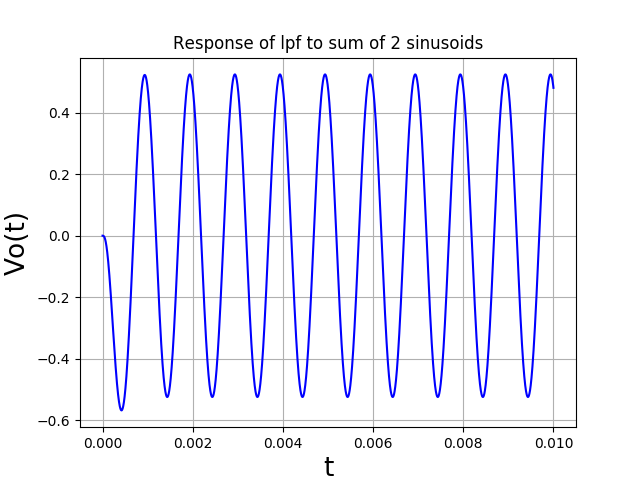
\includegraphics[scale=0.5]{img5.png}
   	\label{fig:32}
   \end{figure}
\begin{figure}[!tbh]
   	\centering
   	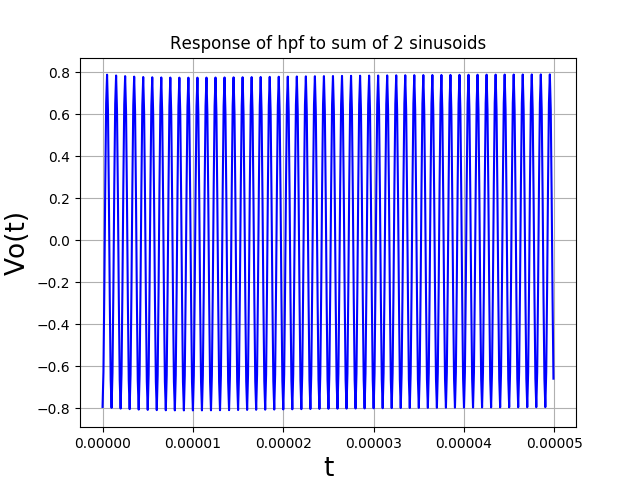
\includegraphics[scale=0.5]{img6.png}
   	\label{fig:32}
   \end{figure}
{
As expected we observe the lpf only allows the low frequency sinusoid to pass and the hpf only allows the high frequency sinusoid to pass.
Observe the differing time scales in both the images.
}
\subsection{Response to damped sinusoids}
{
We input damped sinusoidal inputs of low and high frequencies to observe how the filters will respond.
}
\begin{minted}{python3}
#Response of of lpf and hpf to damped sinusoids
#Damping factor is chosen such that
#damping is visible in the time frame.
#Both low and high freq inputs are given.
damping_factor = 100
t = np.arange(0,1e-2,1e-7)
t,vtd,svec = sp.lsim(Hh,
    np.exp(-damping_factor*t)*(np.cos(2*10**6*np.pi*t)),t)
plotter(0,t,vtd,r"t",r'Vo(t)',
       plt.plot,title ='Response of hpf to high freq damped sinusoid')


t = np.arange(0,1e-2,1e-7)
t,vtd,svec = sp.lsim(Hl,
    np.exp(-damping_factor*t)*(np.cos(2*10**6*np.pi*t)),t)
plotter(1,t,vtd,r"t",r'Vo(t)',
       plt.plot,title ='Response of lpf to high freq damped sinusoid')


t = np.arange(0,1e-2,1e-7)
t,vtd,svec = sp.lsim(Hl,
    np.exp(-damping_factor*t)*(np.sin(2000*np.pi*t)),t)
plotter(2,t,vtd,r"t",r'Vo(t)',
       plt.plot,title ='Response of lpf to low freq damped sinusoid')


t = np.arange(0,1e-2,1e-7)
t,vtd,svec = sp.lsim(Hh,
    np.exp(-damping_factor*t)*(np.sin(2000*np.pi*t)),t)
plotter(3,t,vtd,r"t",r'Vo(t)',
       plt.plot,title ='Response of hpf to low freq damped sinusoid')
plt.show()
\end{minted}
\begin{figure}[!tbh]
   	\centering
   	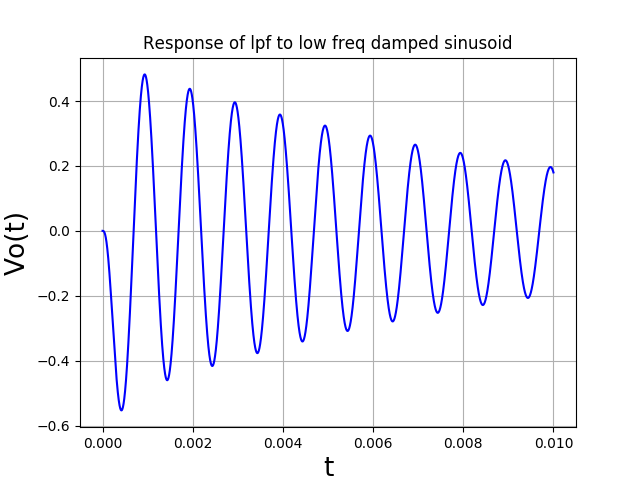
\includegraphics[scale=0.5]{img7.png}
   	\label{fig:32}
   \end{figure}
\begin{figure}[!tbh]
   	\centering
   	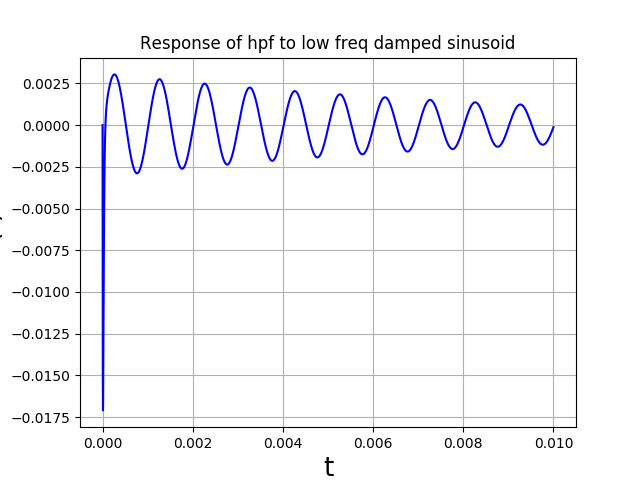
\includegraphics[scale=0.5]{img8.png}
   	\label{fig:32}
   \end{figure}
\begin{figure}[!tbh]
   	\centering
   	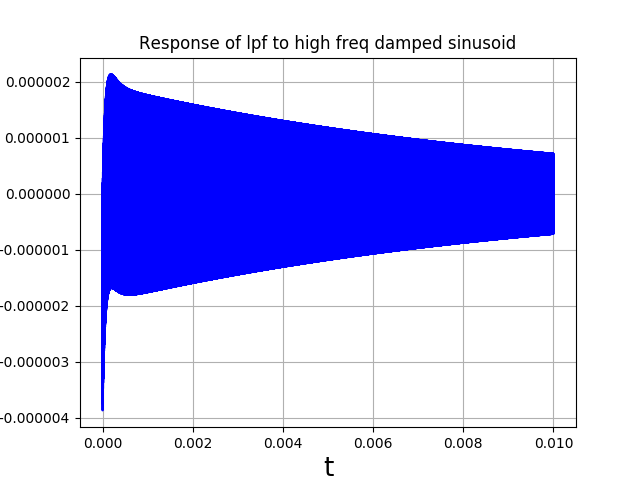
\includegraphics[scale=0.5]{img9.png}
   	\label{fig:32}
   \end{figure}
\begin{figure}[!tbh]
   	\centering
   	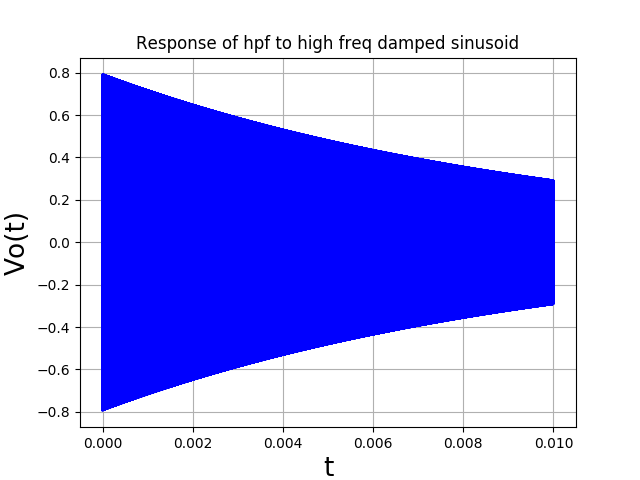
\includegraphics[scale=0.5]{img10.png}
   	\label{fig:32}
   \end{figure}

{
The low frequency sinusoid when passed through the high pass filter shows much quicker decay than when passed through the low pass filter.
This is expected as the hpf acts in a damping fashion to the low frequency sinusoid.
The opposite is observed for the high frequency sinusoid.

}




\section{Conclusions}
\begin{itemize}
\item We  analyzed analog filters in the Laplace domain using sympy.
\item We used the scipy signals to analyse the response to various input signals.
\item We plotted graphs to understand the above.
\end{itemize}

\end{document}
